\documentclass[16pt]{beamer}
\usepackage[utf8]{inputenc}

\title{Rien à cacher}

\usetheme{default}

\usepackage[utf8]{inputenc}
\usepackage{amsmath}
\usepackage{amsfonts}
\usepackage{amssymb}
\usepackage{pgf}
\usepackage{color}
\usepackage[frenchb]{babel}
\usepackage{amssymb}
\usepackage{hyperref}

\usefonttheme{default}
\usepackage{DejaVuSans}
%\usepackage[sfdefault]{FiraSans} %% option 'sfdefault' activates Fira Sans as the default text font
\usepackage[T1]{fontenc}
\renewcommand*\oldstylenums[1]{{\firaoldstyle #1}}


\setbeamertemplate{navigation symbols}{} %remove navigation symbols

\author{Cédric Jeanneret (aka \href{https://www.twitter.com/SwissTengu}{@SwissTengu})}
\institute{\href{https://www.ethack.org/}{EthACK.org}}
\date{\today}

\definecolor{linecolor}{HTML}{4d4c4c}

\setbeamercolor{linecolor}{fg=white,bg=linecolor}

\setbeamertemplate{headline} {
	\begin{beamercolorbox}[wd=\paperwidth,dp=8pt,ht=12pt,leftskip=.29cm,rightskip=.29cm]{linecolor}
	\hfill
	\hypersetup{
		colorlinks=true,
		linkcolor=white,
		urlcolor=white,
	}
	\insertinstitute
	\end{beamercolorbox}%
}

\setbeamertemplate{footline}{%
	\begin{beamercolorbox}[wd=\paperwidth,dp=9pt,ht=0.4cm,leftskip=.29cm,rightskip=.3cm]{linecolor}
	\pgfputat{\pgfxy(0.455,-0.315)}{\pgfbox[center,base]{
\includegraphics[width=1.5cm]{../common/logo_537.png}}}
	\hfill
	\inserttitle
	\end{beamercolorbox}%
}


\hypersetup{
	colorlinks=true,
	linkcolor=blue,
	urlcolor=blue,
	pdfborderstyle={/S/U/W 1},
	pdfborder=0 0 1,
	linkbordercolor={0 0 0},
	urlbordercolor={0 0 0},
}


\begin{document}

{
\setbeamertemplate{footline}{%
	\begin{beamercolorbox}[wd=\paperwidth,dp=8pt,ht=12pt,leftskip=.29cm,rightskip=.3cm]{linecolor}
	\hfill
	\inserttitle
	\end{beamercolorbox}%
}

% center first slide — not a title, but almost
{
\centering
\begin{frame}

EthACK
\vspace{0.5cm}

The Swiss Privacy Basecamp 
\vspace{0.5cm}


\includegraphics[width=4cm]{../common/logo_537.png}

\end{frame}
}
}

\begin{frame}{EthACK ?}
\begin{itemize}
	\item Éthique
	\item État
	\item ACKnowledgement (reconnaissance)
	\item Hacking (éthique, évidemment)
	\item …
\end{itemize}
\end{frame}

\begin{frame}{Pourquoi ?}
\begin{itemize}
	\item Notre gouvernement ne s'intéresse pas (ou peu) au sujet
	\item Les sociétés privées nous fichent à notre insu
	\item Personne ne sait où sont leurs données, qui les traitent, à quoi elles servent
\end{itemize}
\end{frame}


\begin{frame}
  \titlepage
\end{frame}

\begin{frame}
{Notion de données personnelles}
\begin{itemize}
\item Ce que dit la Loi (suisse) : \newline
\textit{toutes les informations qui se rapportent à une personne identifiée ou identifiable;} \newline
 \vspace{0.1cm} \newline \tiny{RS235.1, article 3}\newline
\end{itemize}
\end{frame}

\begin{frame}
{Notions de données sensibles}
\begin{itemize}
\item Ce que dit la Loi (suisse) : \newline données \textit{sensibles}, sur :
\begin{itemize}
\item les opinions ou activités religieuses, philosophiques, politiques ou syndicales,
\item la santé, la sphère intime ou l'appartenance à une race,
\item des mesures d'aide sociale,
\item des poursuites ou sanctions pénales et administratives;
\end{itemize}
\end{itemize}
\end{frame}

\begin{frame}
{À quoi servent les données personnelles ?}
\begin{itemize}
\item À nous définir en tant qu'individu
\item À nous démarquer de la masse
\item À nous regrouper
\end{itemize}
\end{frame}

\begin{frame}
{Mais à quoi ça sert ? Pourquoi les protéger ?}
\begin{itemize}
\item Décisions (crédit, logement, emploi, etc)
\item Profits (marché des données personnelles, etc)
\item Renseignements (militaire, police, …)
\end{itemize}
\end{frame}

\begin{frame}
\centering
Le tout la plupart du temps à votre insu, sans votre consentement !
\end{frame}

\begin{frame}
\centering

\includegraphics[height=\textheight,keepaspectratio]{./kidding.jpg}
\end{frame}

\begin{frame}
{Sérieusement… ?}
\centering 
Des sociétés privées sont intéressées par vos habitudes d'achat.\newline
\vspace{0.5cm} \newline
Des sociétés privées sont intéressées par vos centres d'intérêts. \newline
\vspace{0.5cm} \newline

Et vendront ou achèteront ces informations. Oui, à votre insu.
\end{frame}

\begin{frame}
{Collecte des données}
\begin{itemize}
\item Par \textit{un} État
\item Par des sociétés privées
\item Depuis le pays d'habitation
\item Depuis des pays étrangers
\end{itemize}
\end{frame}

\begin{frame}
{Qui en profite ?}
\begin{itemize}
\item \textit{Un} État
\item Les entreprises
\item<+-> …
\item<+-> En tous cas pas vous ! 
\end{itemize}
\end{frame}

\begin{frame}
\centering

\includegraphics[height=\textheight,keepaspectratio]{./seriouscatcover.jpg}
\end{frame}

\begin{frame}
{Sauf…}
Si vous aimez avoir :
\begin{itemize}
\item Publicité ciblée
\item Offres ciblées
\item Votre profile complet vous ne savez où
\end{itemize}
\end{frame}

\begin{frame}
{Pourquoi se protéger ?}
\begin{itemize}
\item Vous ne savez pas qui possède vos données
\item Vous ne savez pas quelles données ils possèdent
\item Vous ne savez pas ce qu'ils en font
\end{itemize}
\end{frame}

\begin{frame}
{Et alors ?!}
\centering
\Huge{Je n'ai rien à cacher !}
\end{frame}

\begin{frame}
{Origine de cette phrase…}
\centering
\Large{Vous n'avez rien à craindre si vous n'avez rien à cacher}
\newline
\vspace{1cm}\newline
\tiny{(Ministre du III$^{eme}$ Reich à l'Éducation du peuple et à la Propagande — Joseph Goebbels)}\newline\vspace{0.5cm}\newline
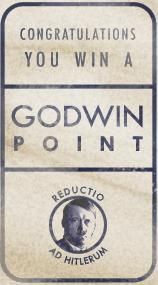
\includegraphics[height=2.5cm]{./godwin.jpg}
\end{frame}

\begin{frame}
{Pourquoi se protéger ?}
\begin{itemize}
\item Mise à jour des données \newline
\item Données pour des décisions à votre encontre
\item Les décisions peuvent se baser sur des données erronées ou dépassées
\end{itemize}
\end{frame}

\begin{frame}
{Exemple de décisions}
Un logement peut vous être refusé à cause de données fausses/dépassées\newline
\vspace{1cm}\newline
Un crédit peut vous être refusé de même
\end{frame}

\begin{frame}
\centering

\includegraphics[height=\textheight,keepaspectratio]{./isee.jpg}
\end{frame}

\begin{frame}
{Qui ?}
\begin{itemize}
\item Poursuites : plus de 100 entreprises privées
\item Revenus : Plus de 250 entreprises privées
\item Situation financière : plus de 170 entreprises privées
\end{itemize}
\vspace{0.5cm}
\tiny{\href{https://www.datareg.admin.ch/WebDatareg/search/search.aspx?lang=fr}{Source: PFPDT}}
\end{frame}

\begin{frame}
{Qui ? (données sensibles)}
\begin{itemize}
\item Santé : plus de 300 entités privées
\item Origine : plus de 50 entités privées
\item Religion : plus de 50 entités privées
\end{itemize}
\vspace{0.5cm}
\tiny{\href{https://www.datareg.admin.ch/WebDatareg/search/search.aspx?lang=fr}{Source: PFPDT}}
\end{frame}

\begin{frame}
{Pourquoi ?}
\begin{itemize}
\item Service après-vente
\item Ciblage publicitaire
\item "Prises de décisions"
\begin{itemize}
\item Crédit
\item Logement
\item …
\end{itemize}
\item …
\end{itemize}
\end{frame}

\begin{frame}
{Et l'État ?}
\begin{itemize}
\item Protection de la population
\begin{itemize}
\item Police
\item Terrorisme
\item …
\end{itemize}
\end{itemize}
\end{frame}

\begin{frame}
\centering

\includegraphics[height=\textheight,keepaspectratio]{./surveillance.png}
\end{frame}

\begin{frame}
{Se protéger, mais comment ?}
\begin{itemize}
\item Hygiène
\item Chiffrer
\item Trier
\item Contrôler
\end{itemize}
\end{frame}

{
\setbeamertemplate{footline}{%
	\begin{beamercolorbox}[wd=\paperwidth,dp=8pt,ht=12pt,leftskip=.29cm,rightskip=.3cm]{linecolor}
	\hfill
	\inserttitle
	\end{beamercolorbox}%
}
{
\centering
\begin{frame}
{Questions ?}

\href{https://ethack.org/}{https://ethack.org/} \\
\vspace{0.3cm}
\href{https://www.twitter.com/EthACK_org}{@EthACK\_org} on Twitter \\
\vspace{0.3cm}
\href{https://www.facebook.com/ethack.org}{ethack.org} on Facebook

\vspace{0.5cm}


\includegraphics[width=4cm]{../common/logo_537.png}
\end{frame}
}
}

\end{document}